\section{System Setup}
The end system has two arrays, each with three microphones mounted on vetices of a $20$ cm equilateral triangle. A micro-controller is also attached to one of the vertices. Fig~\ref{fig:setup_array} shows a picture of the array setup. Micro-controller used in this project is \emph{teensy 3.1}. It has $64$k RAM memory and the ADC is capable of sampling at $500$kHz. In this project, the micro-controller collects microphone data on all three channels for $12$ millisecond and then send the recorded data to a computer through USB port for localization. 

\begin{figure}[]
  \centering
  \begin{subfigure}[]{.23\textwidth}
    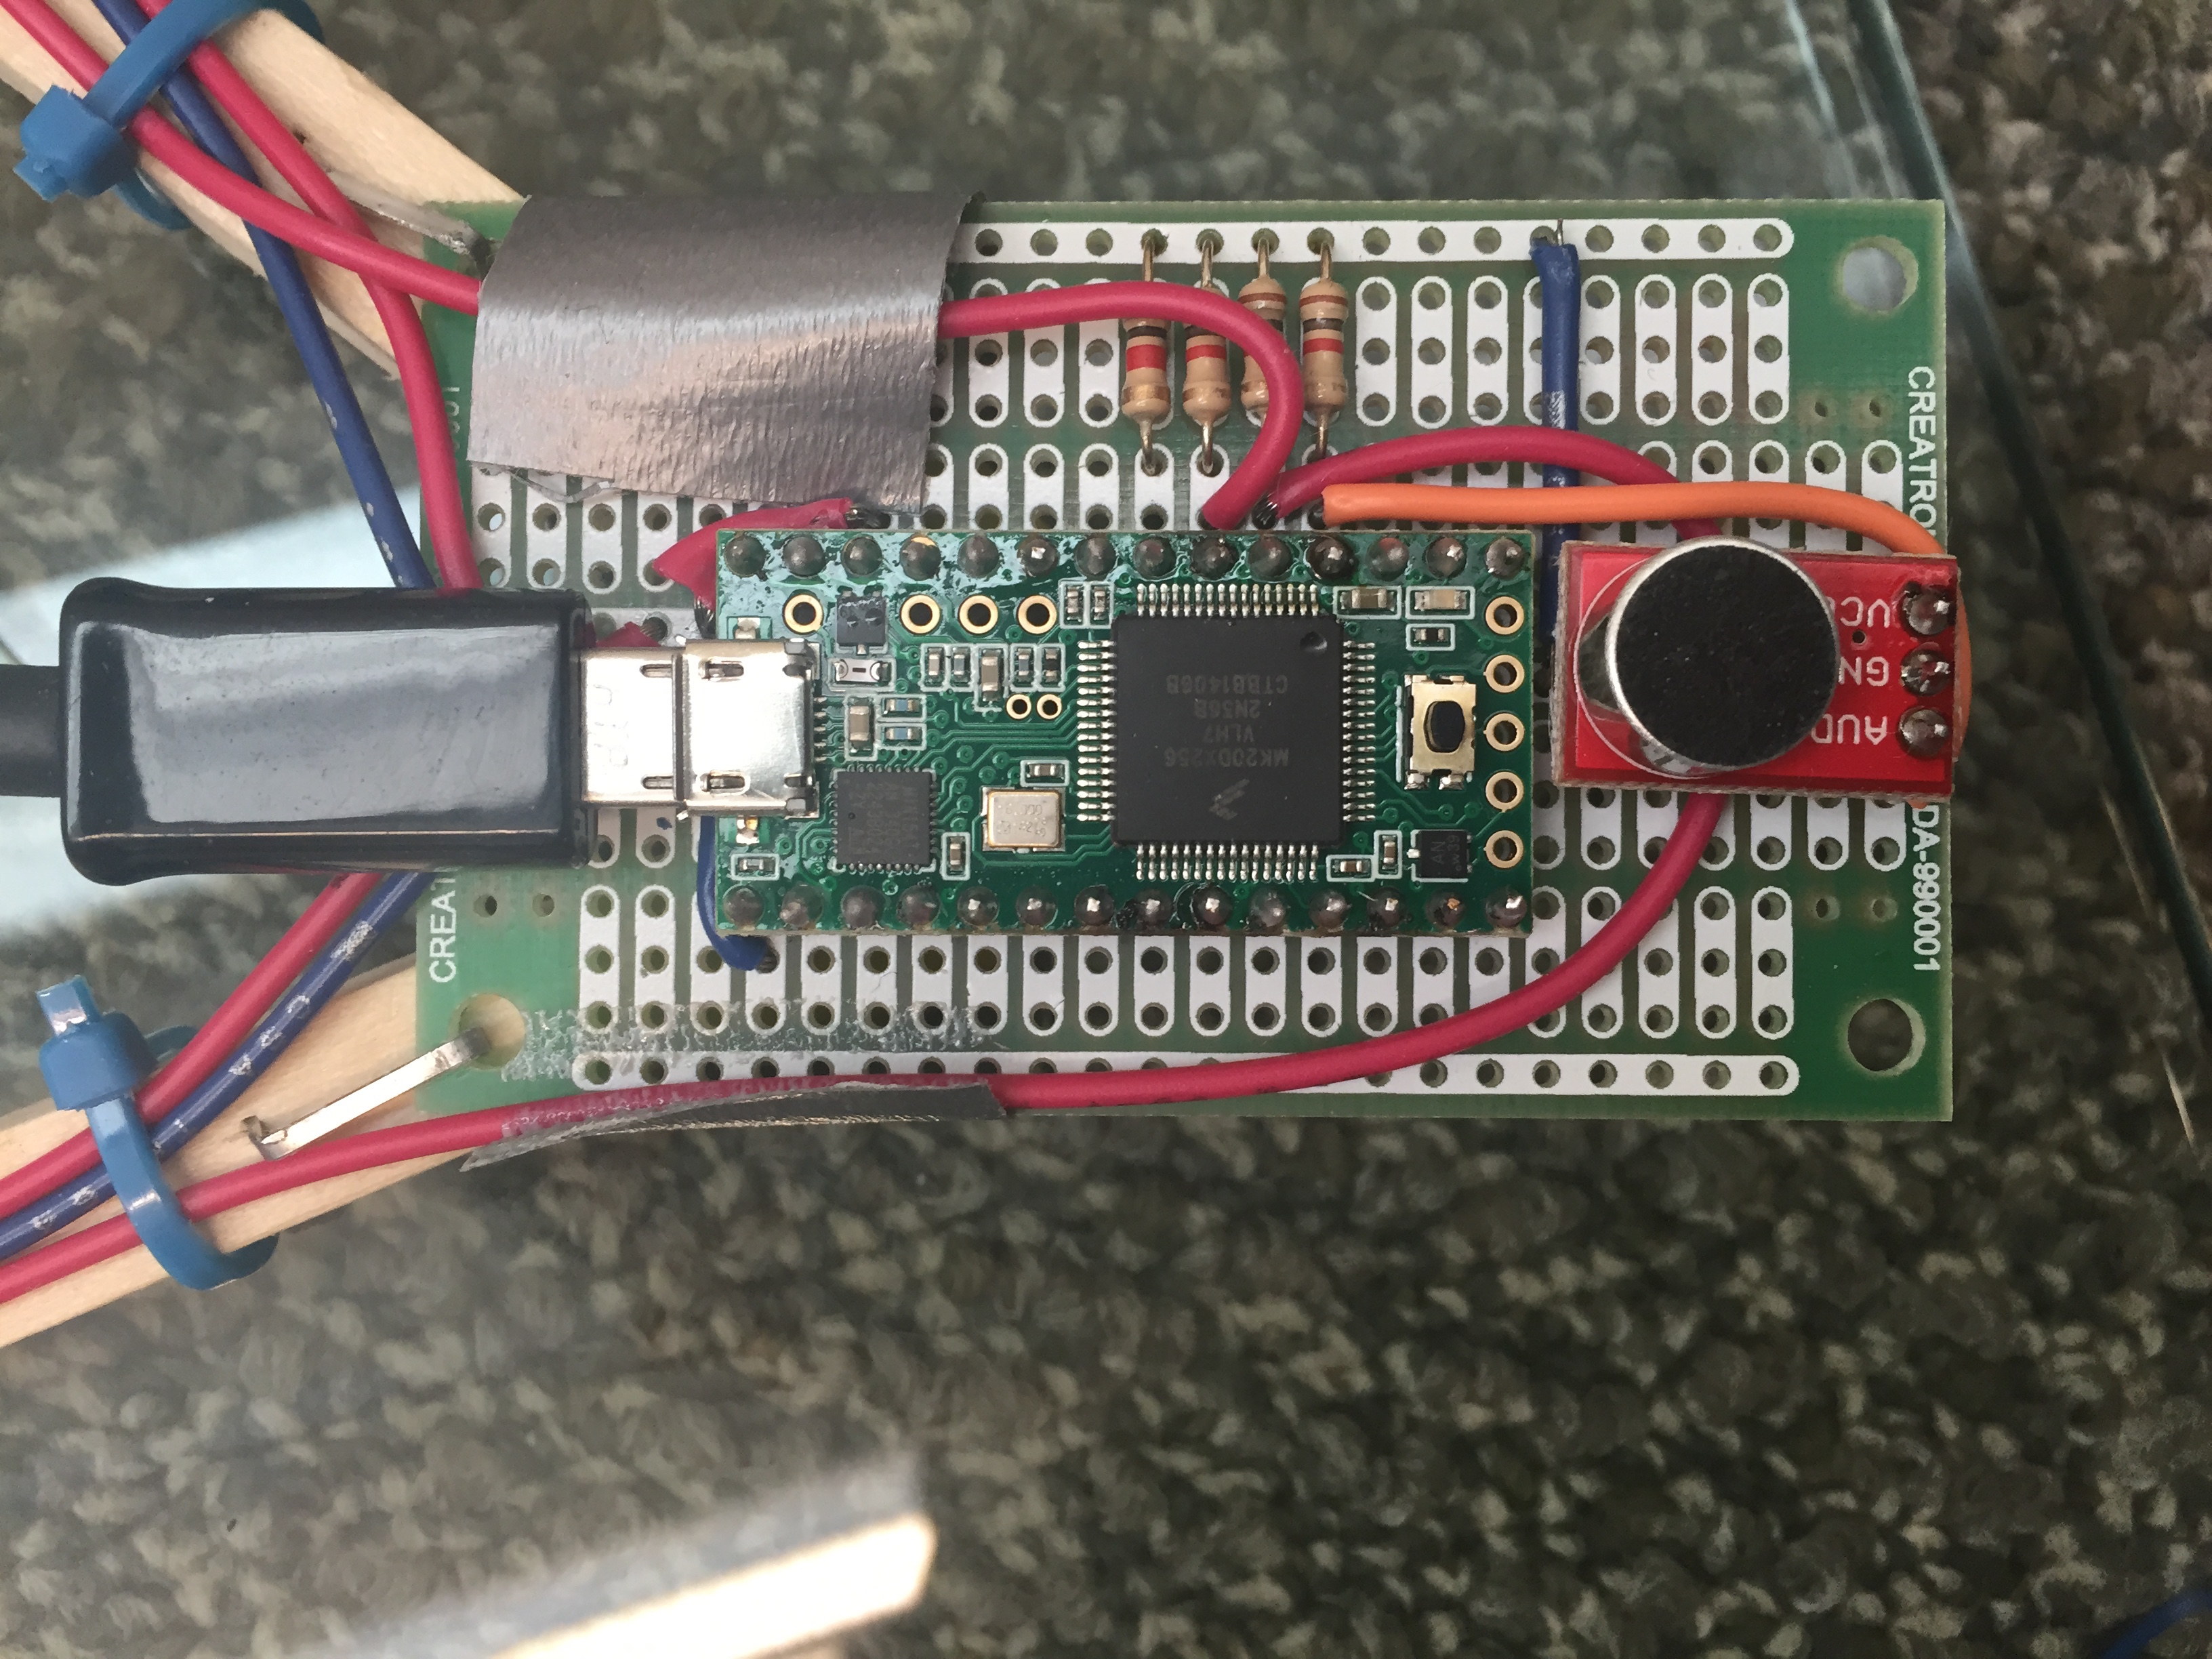
\includegraphics[width=\textwidth]{array_close.JPG}
    \caption{micro-controller}
  \end{subfigure}
  \begin{subfigure}[]{.23\textwidth}
    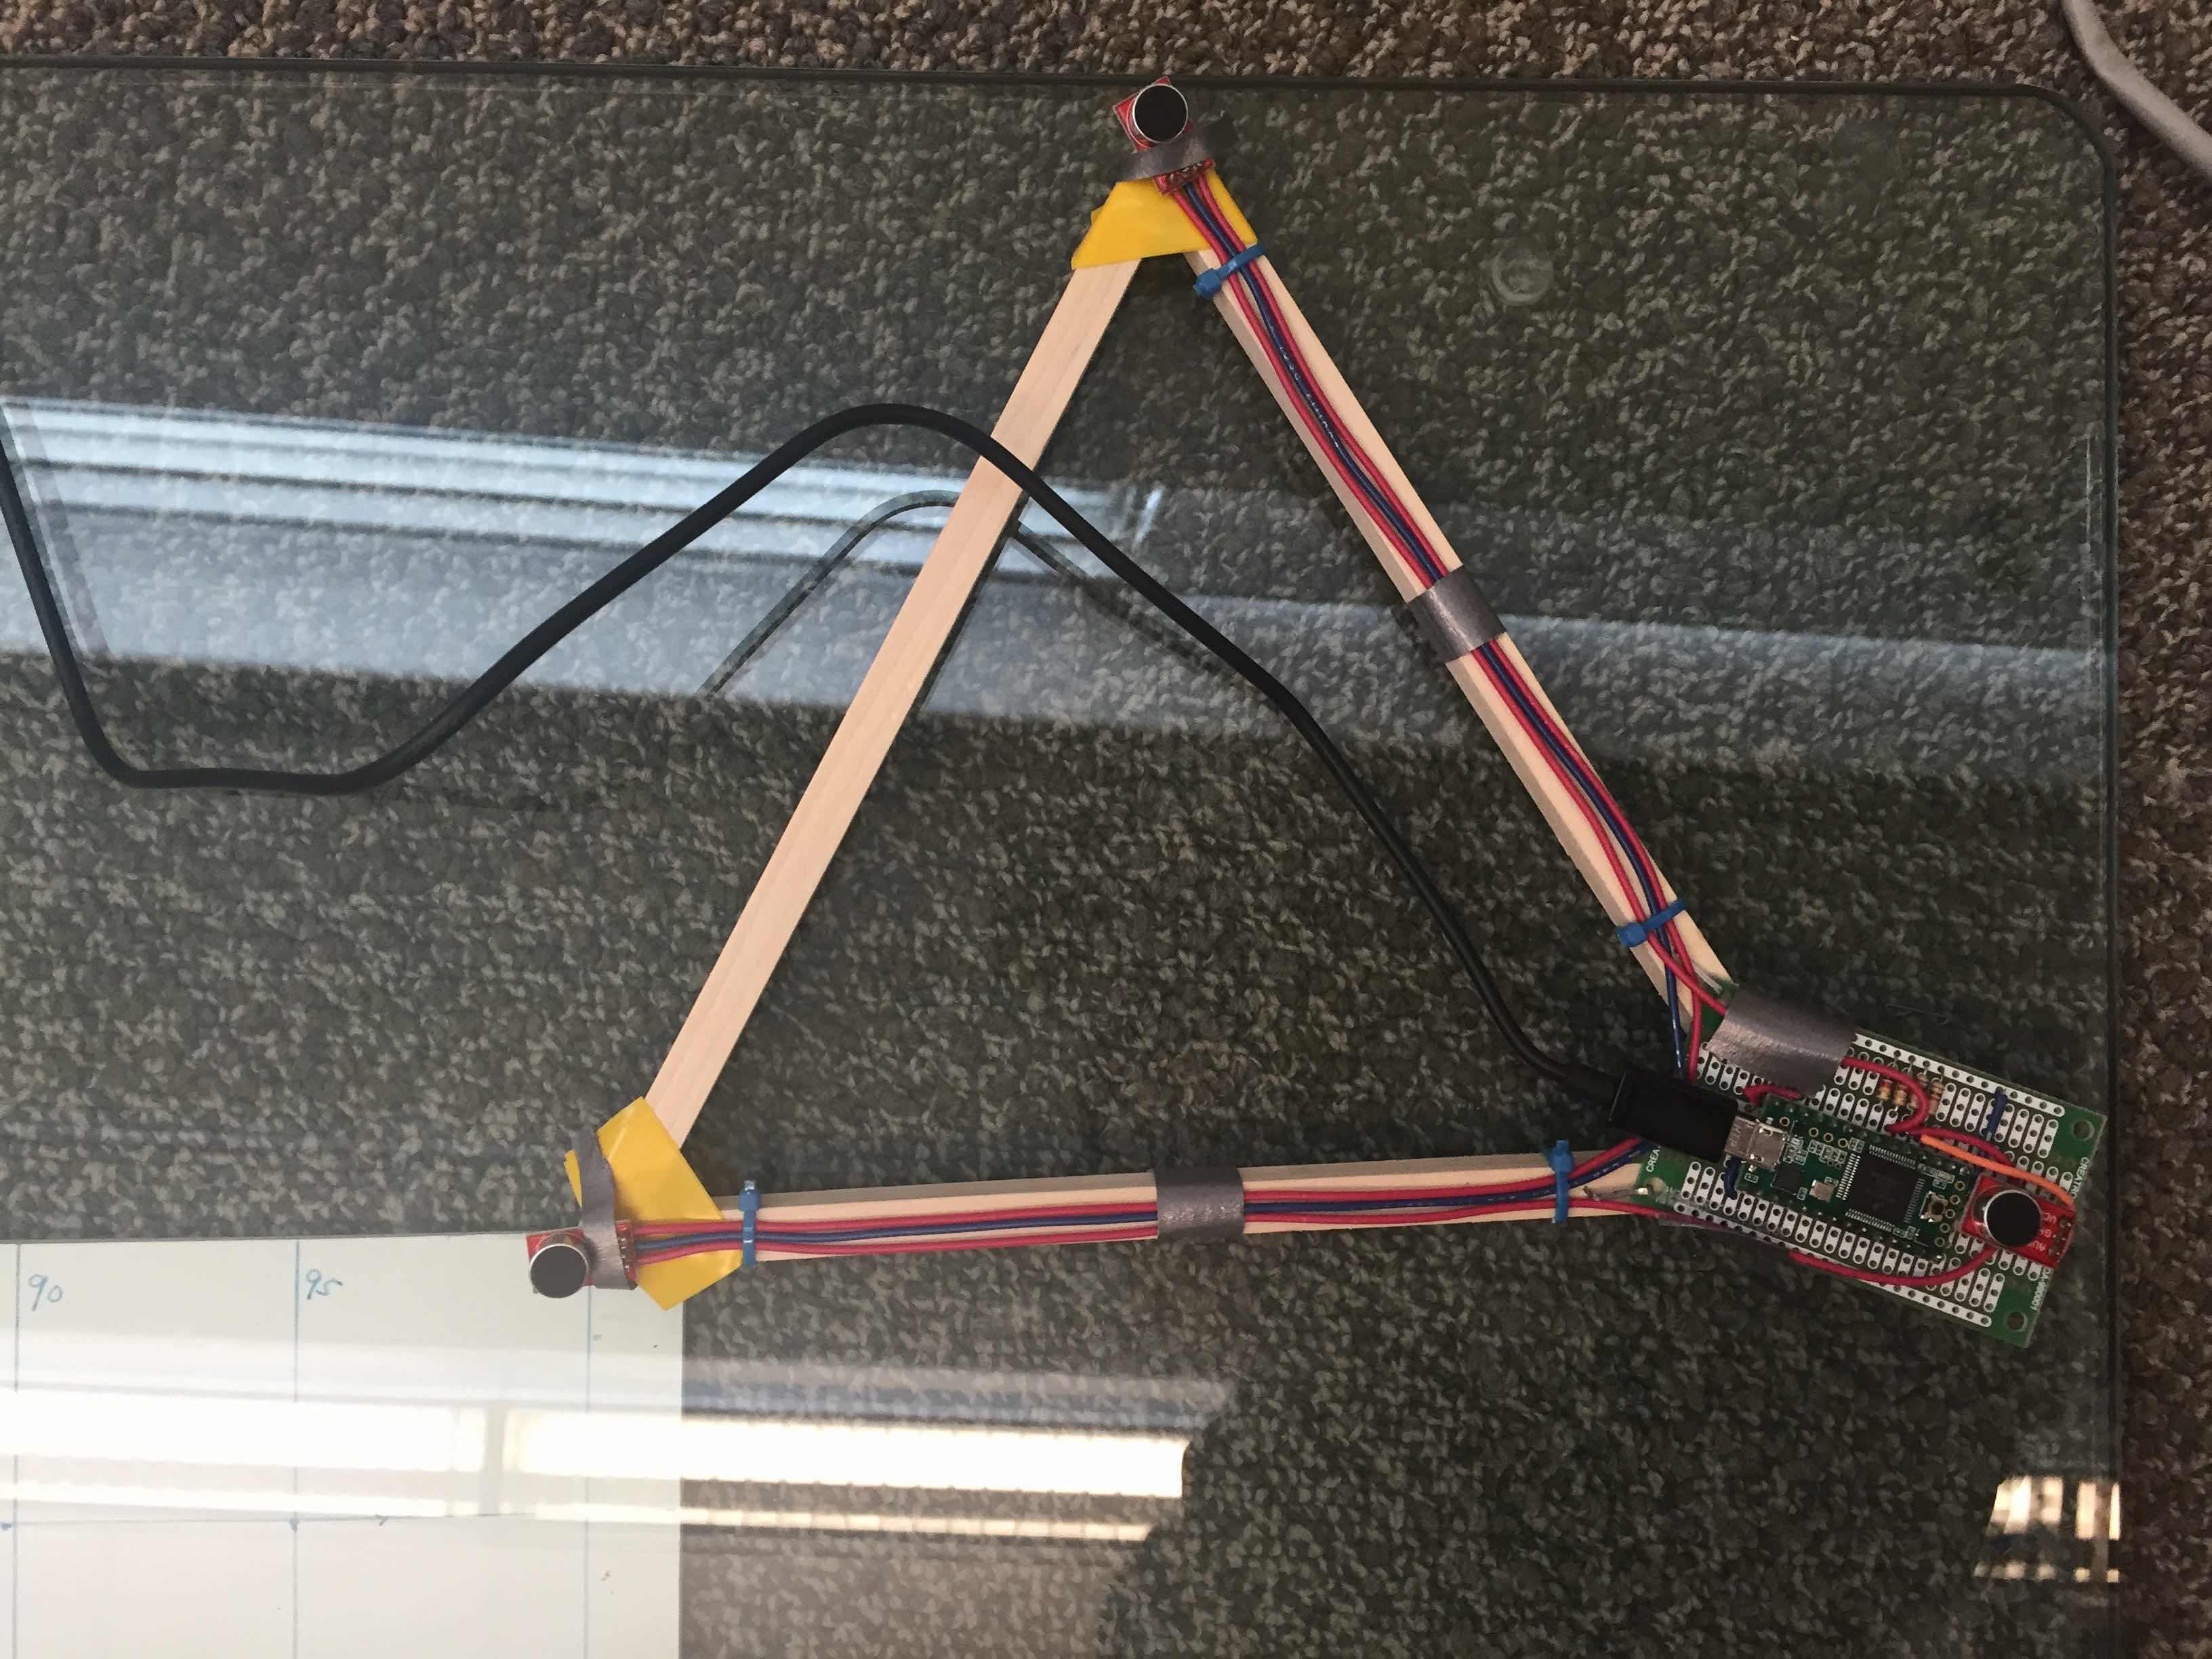
\includegraphics[width=\textwidth]{array.JPG}
    \caption{array}
  \end{subfigure}
  \begin{subfigure}[]{.23\textwidth}
    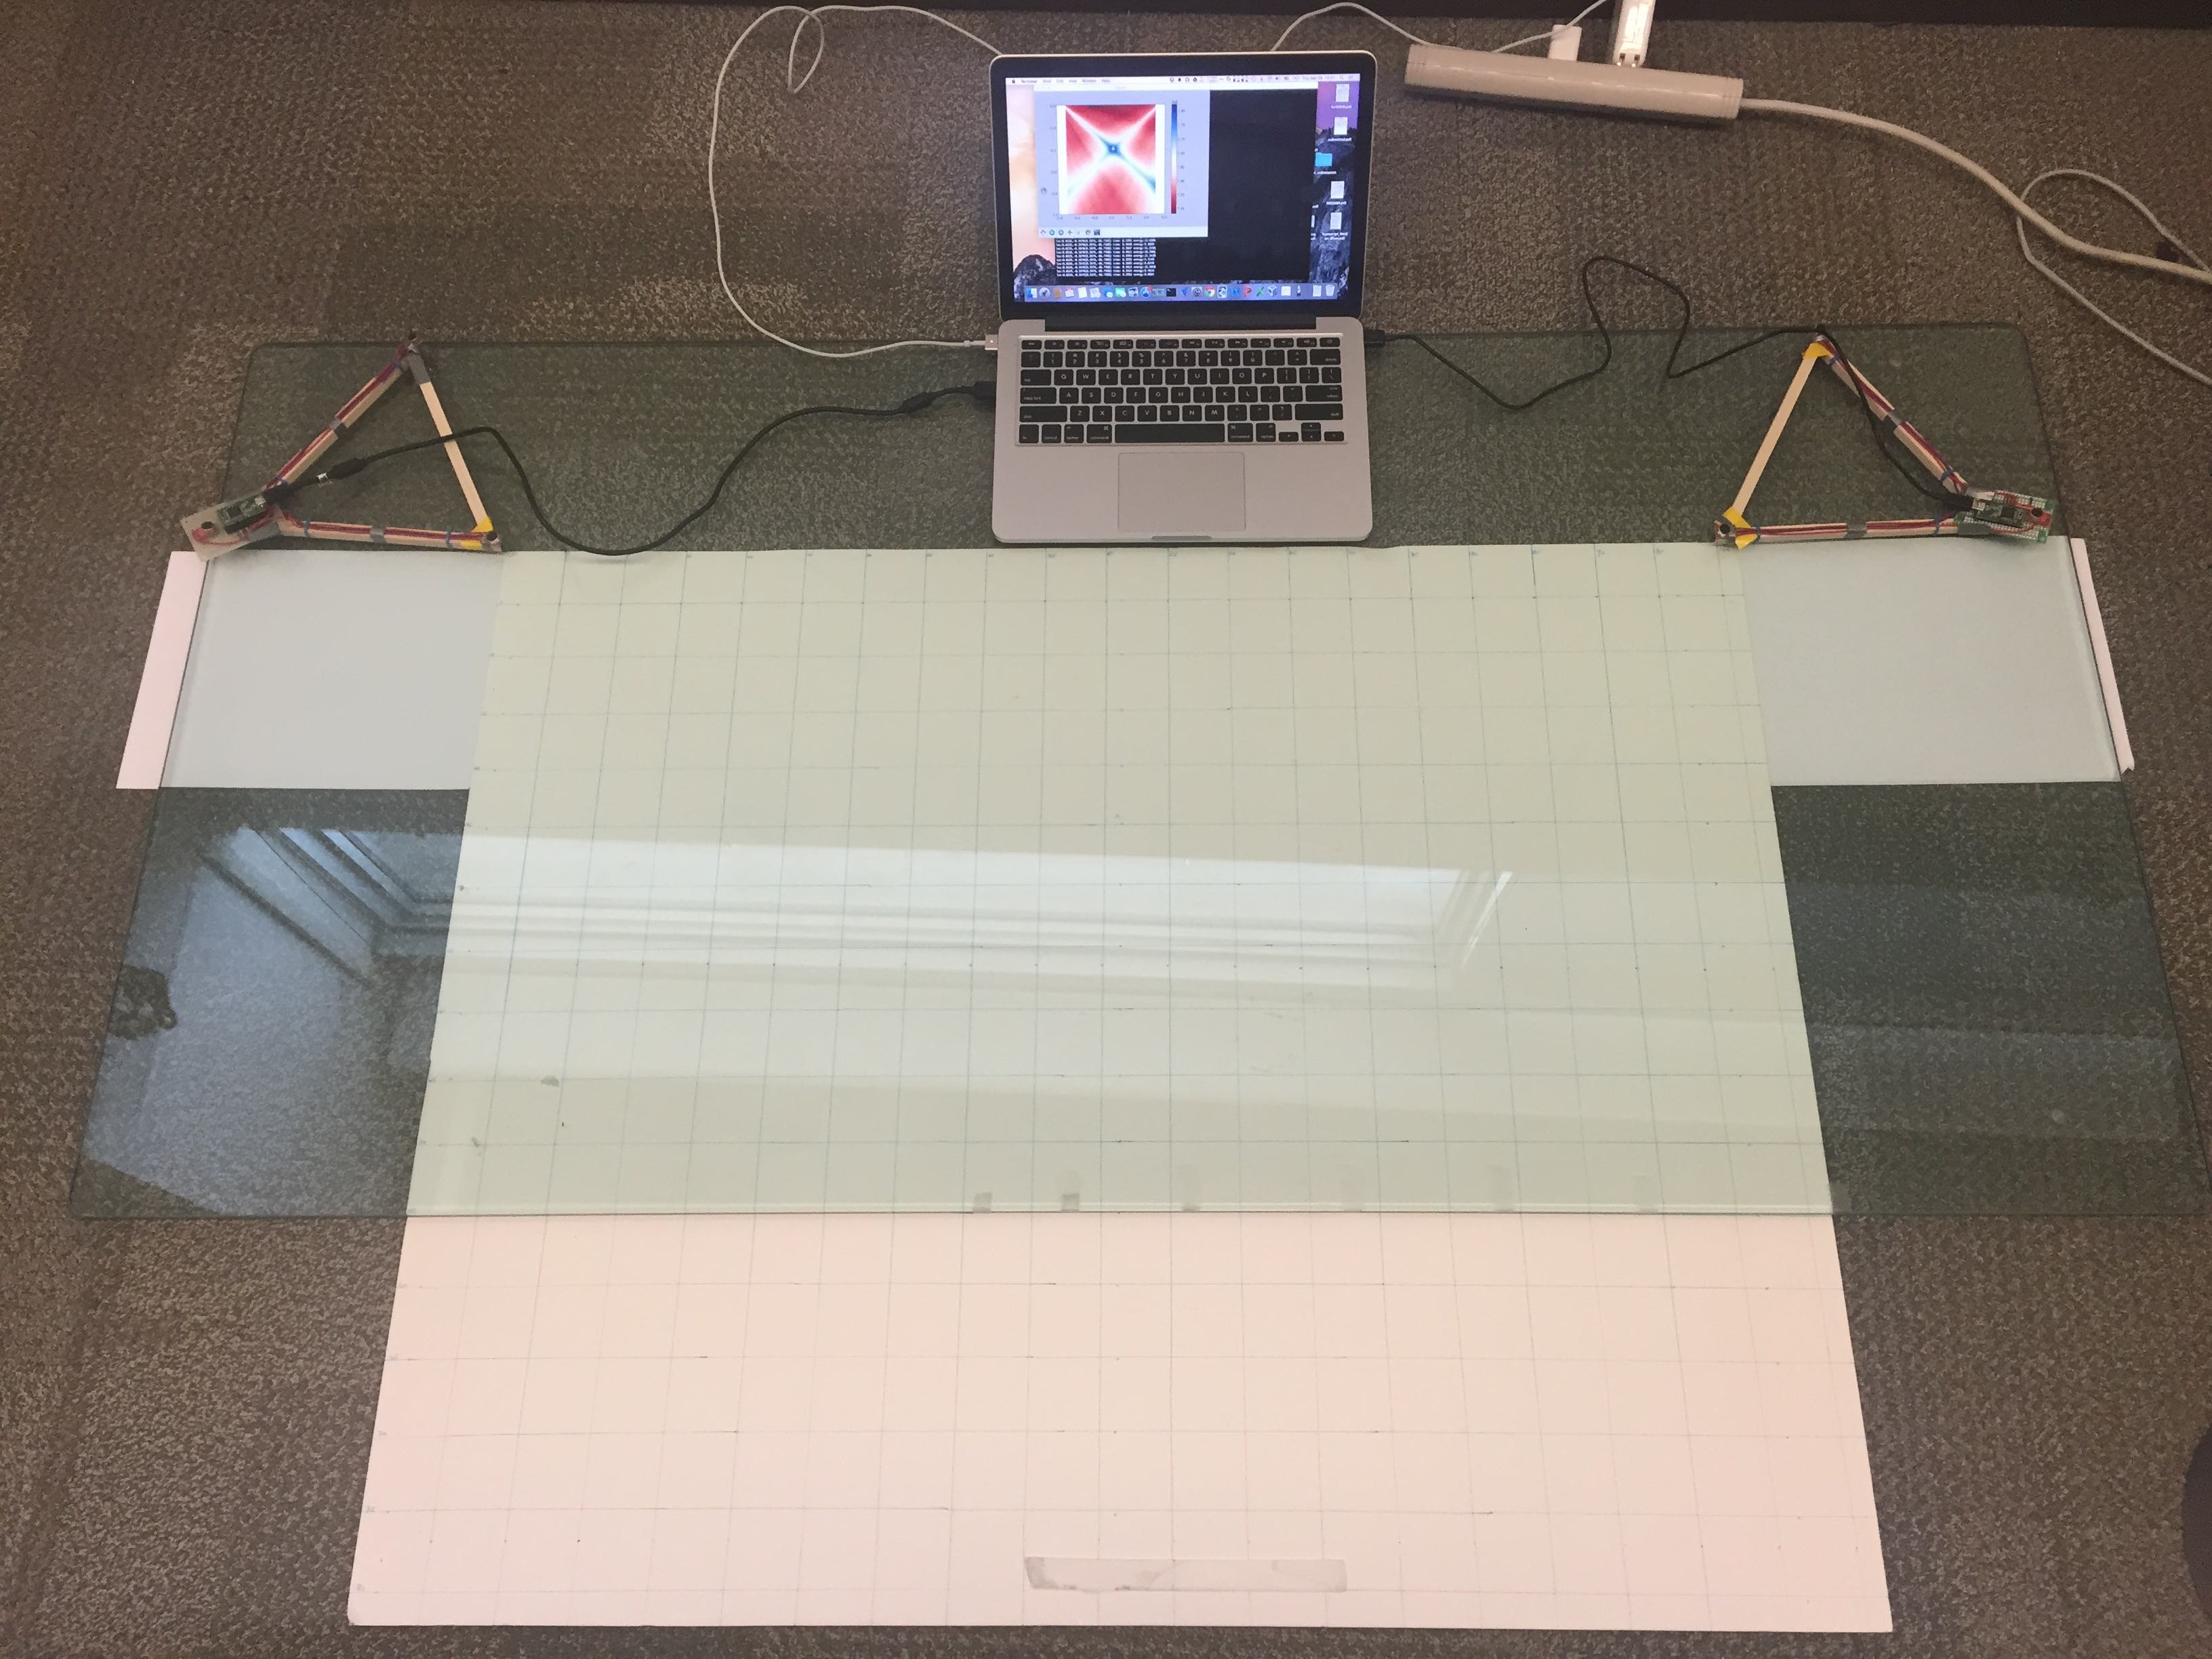
\includegraphics[width=\textwidth]{setup_2.JPG}
    \caption{two arrays}
  \end{subfigure}
  \caption{Localization arrays}
  \label{fig:setup_array}
\end{figure}

To speed up computation for real time localization, instead of searching for $t_0$ that maximizes equation~\ref{eq:gcc}, a grid search in 2D grid is performed. For each point in the grid, the theoretical TDOA to each microphone pair can be precomputed. Then localization resolves to calculating GCC for each microphone pair and performing a lookup for each point in the grid. To further improve localization accuracy, instead of using point estimate for TDOA, a liklihoood map is built. Each entry in GCC output is used as the liklihood for that delay. With three microphones $m_1,m_2,m_3$, there are three microphones pairs: $m_1m_2,m_1m_3,m_2m_3$. Theoretical TDOA from each location $(x,y)$ to each microphone pair is precomputed and stored in $D_{m_1,m_2}(x,y)$, $D_{m_1,m_3}(x,y)$, and $D_{m_2,m_3}(x,y)$. Then the liklihood map can be built as:
\begin{eqnarray*}
  L(x,y) &=& R_{m_1,m_2}(D_{m_1,m_2}(x,y)) + R_{m_1,m_3}(D_{m_1,m_3}(x,y)) \\
 & & +R_{m_2,m_3}(D_{m_2,m_3}(x,y)) 
\end{eqnarray*}
,where $R_{m_1,m_2}(\tau)$,$R_{m_1,m_3}(\tau)$, and $R_{m_2,m_3}(\tau)$ denote GCC output from microphone pairs $m_1m_2,m_1m_3,$ and $m_2m_3$.

Liklihood maps from two arrays can be combined into final liklihood map:
\begin{equation}\label{eq:combine_l}
L(x,y) = L_1(x,y) L_2(x,y)
\end{equation}
, where $L_1(x,y)$ and $L_2(x,y)$ represents the liklihood map from array $1$ and array $2$.

\begin{figure}[]
  \centering
  \begin{subfigure}[]{.23\textwidth}
    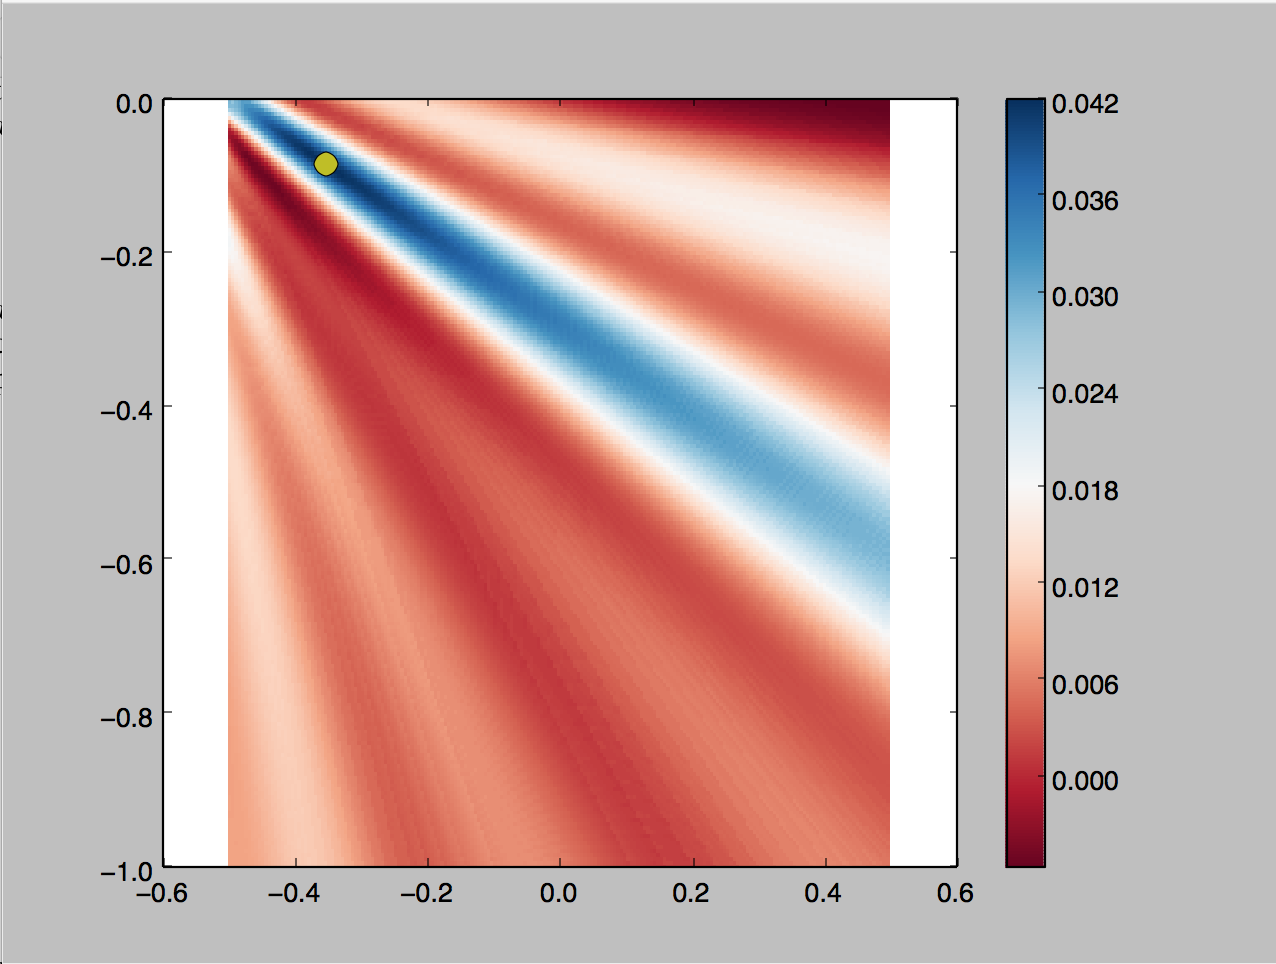
\includegraphics[width=\textwidth]{left.png}
    \caption{localization with only array 1}
    \label{fig:liklihood1}
  \end{subfigure}
  \begin{subfigure}[]{.23\textwidth}
    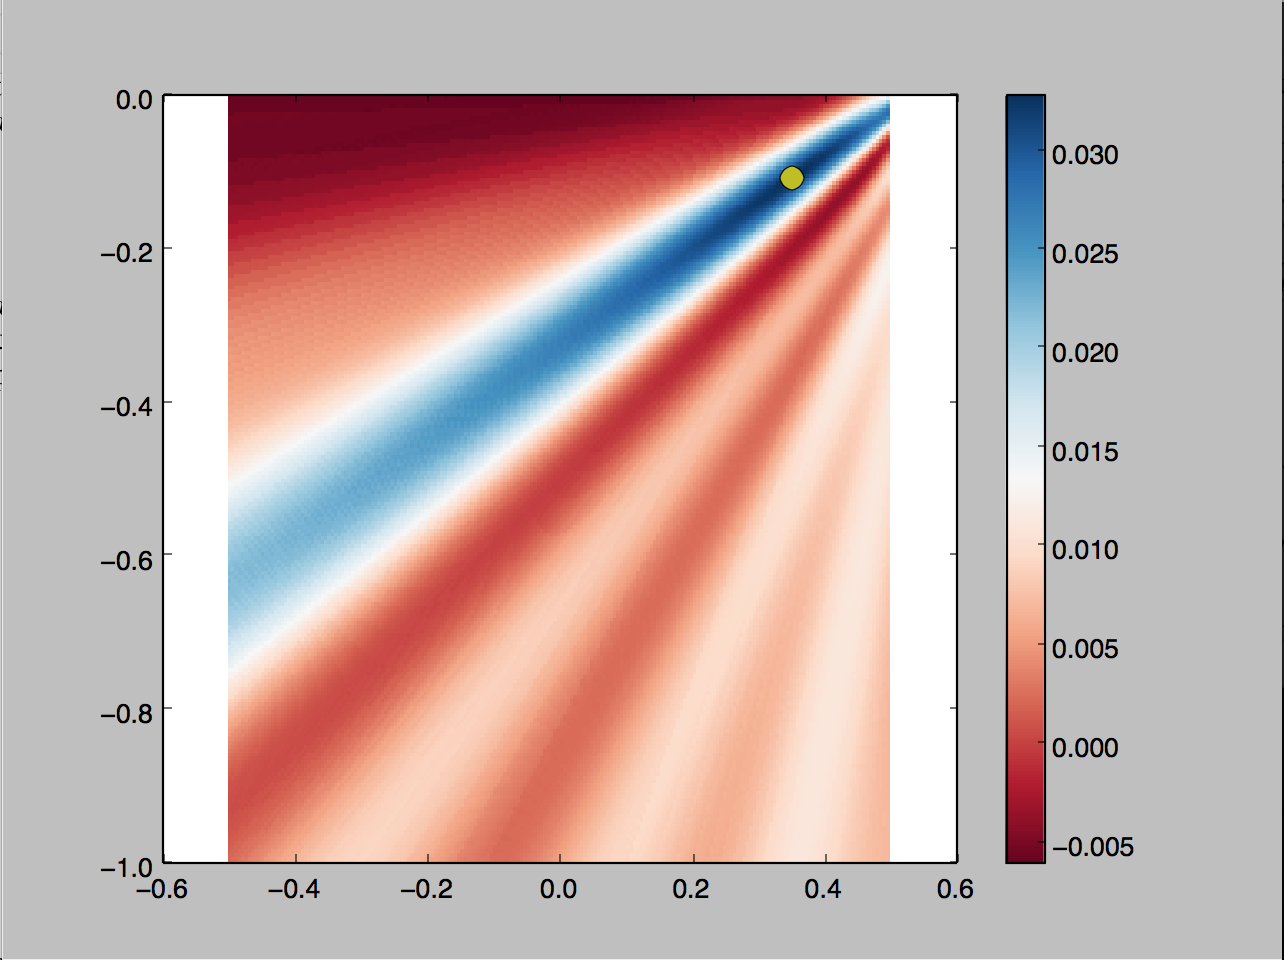
\includegraphics[width=\textwidth]{right.png}
    \caption{localization with only array 2}
    \label{fig:liklihood2}
  \end{subfigure}
  \begin{subfigure}[]{.23\textwidth}
    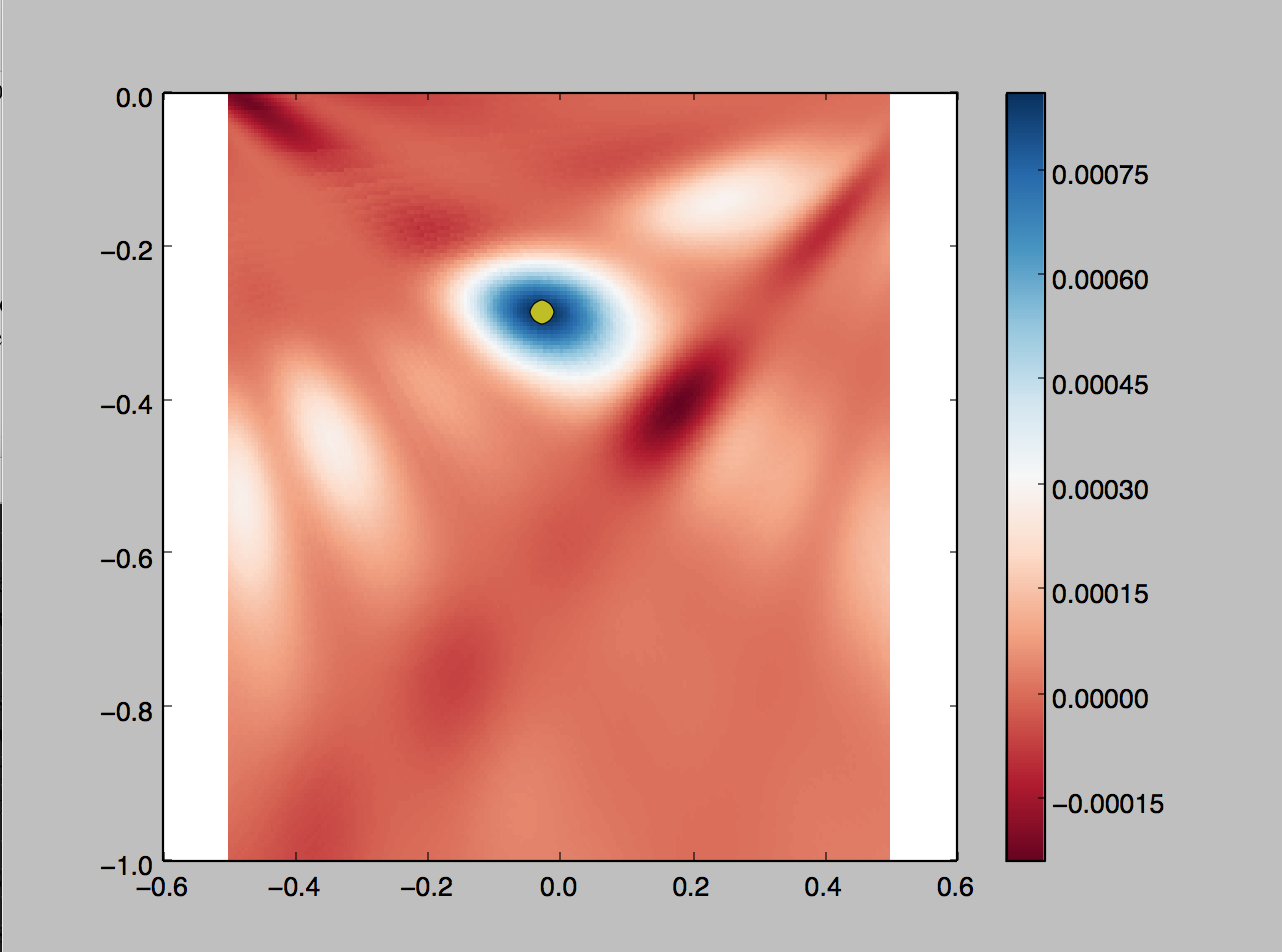
\includegraphics[width=\textwidth]{combined.png}
    \caption{localization with both arrays}
    \label{fig:liklihood3}
  \end{subfigure}
  \caption{Liklihood maps for localizating point at $(0.0,-0.3)$ m}
  \label{fig:liklihood}
\end{figure}


To see the effect of using multiple arrays, fig~\ref{fig:liklihood} shows the individual liklihood map from each array and also the combined liklihood map according to equation~\ref{eq:combine_l}. Individual array gives accurate angle estimate, but has high uncertainty in distance estimate. By combining estimates from two arrays, the angle estimate can be effectively combined to estimate distance.

From a timing point of view, the micro-controller spends $12$ millisecond on sampling microphone data before sending the data to the computer for processing. Sending data through USB port takes another $18$ millisecond, and processing on computer takes around $50$ millisecond. Therefore, the totoal time lag between sound source and localization is around $80$ millisecond.
